\documentclass[a4paper,12pt]{article}

\usepackage[french]{babel}
\usepackage[utf8]{inputenc}
\usepackage{graphicx}
\usepackage{hyperref}
\usepackage{version}
\hypersetup{colorlinks, citecolor=black, filecolor=black, linkcolor=black, urlcolor=black}

\title{Cahier des charges du Projet Nigma}
\author{CrypTeam : LAPOTRE Guillaume (\texttt{lapotr\_g}) \and GANIVET Justin (\texttt{ganive\_j}) \and LADEVIE Stéphane (\texttt{ladevi\_s}) \and GISLAIS Sébastien (\texttt{gislai\_s})}
\pagestyle{myheadings}
\date{21 novembre 2008}

\begin{document}
%<<<<<<< .mine
	\markright{Cahier des charges de la CrypTeam}
	\maketitle{}
	\newpage
  	\tableofcontents
	\newpage
	\part{Introduction}
	%introduction rapide
        \section {Présentation de la CrypTeam}
        \section {Présentation individuelle}
        \subsection{Guillaume LAP\^{O}TRE}
Actuellement étudiant en Info-spé à EPITA, j'entame avec réjouissance ce fabuleux projet à la fois utile et pédagogique. En effet, la cryptographie m'a toujours attiré. Mais je n'avais jamais l'occasion de m'y interressé de plus près. La stéganographie n'était pas mon idée mais je l'ai trouvé assez interressante.
        \subsection{Justin GANIVET}
        \subsection{Stéphane LADEVIE}
        \subsection{Sébastien GISLAIS}
	\newpage
\begin{comment}
	\part{\'{E}tat de l'art}
		La cryptographie et la stéganographie sont deux techniques extrêmement ancienne permettant de transmettre des informations uniquement aux personnes voulues.
=======
\markright{Cahier des charges de la CrypTeam}
\maketitle{}
\tableofcontents
\newpage
\part{Introduction}
%introduction rapide
%>>>>>>> .r17

\section {Présentation de la CrypTeam}

\section {Présentation individuelle}

\subsection{Guillaume LAPOTRE}

\subsection{Justin GANIVET}

\subsection{Stéphane LADEVIE}

\subsection{Sébastien GISLAIS}

\newpage
\end{comment}
\part{\'{E}tat de l'art}
La cryptographie et la stéganographie sont deux techniques extrêmement ancienne permettant de transmettre des informations uniquement aux personnes voulues.

La cryptographie protège le message en le chiffrant, c'est-à-dire en le rendant incompréhensible sans connaitre l'algorithme de cryptage. On peut citer comme procédé de cryptage historique le chiffre de César qui décale l'alphabet de n rang suivant le chiffre choisi (ainsi si le chiffre choisi est 3, l'alphabet sera : DEFGHI\dots{}ZABC).

La stéganographie consiste à cacher le message à transmettre plutot que de le chiffrer. Comme exemple historique on peut citer un procédé utilisé par César, il écrivait sur le crane d'un esclave un message puis attendait que les cheveux de cet esclave repoussent puis il envoyait l'esclave à la personne à qui le message était destiné. Il suffisait donc de raser l'esclave pour récupérer le message.

Cepandant, la stéganographie ainsi que la cryptographie étaient utilisée quasiment uniquement par les militaires avant la fin de la Seconde Guerre Mondiale. Depuis, il y a énormément d'application civile au chiffrement.

\section{Cryptographie}

\subsection{Cryptage par substitution}

Le cryptage par substitution  est une des technique les plus basique et les plus ancienne de chiffrement. Le chiffre de César est une technique de cryptage par substitution. Il existe plusieurs types de substitution pour chiffrer des données.

\subsubsection{Le cryptage par substitution mono-alphabétique}

On remplace chaque lettres de l'alphabet par une autre lettre. Ainsi pour la première lettre il y a 26 possibilités, pour la seconde 25 possibilités etc\dots{} Il existe donc $26!$ façons de coder distinctes. L'inconvénient de la substitution mono-alphabétique est qu'il faut se souvenir de chaque substitutions pour chaques lettres. L'autre inconvénient est qu'en connaissant la langue du message codé on peut relativement facilement déchiffrer le message en se basant sur la fréquence d'apparition de chaque lettre dans une langue. Par exemple en français la lettre apparaissant le plus souvent est le E, en analysant un texte chiffré avec cette technique de chiffrement, on peut trouver la lettre qui apparait la plus souvent et l'associer donc à la lettre E. Ensuite on utilise le même raisonnement pour toute les autres lettres.

\subsubsection{Le codage par substitution poly-alphabétique}

Le chiffre de Vigenère en est un exemple. On crée un mot qui sert de clé et \og on le colle en dessous du texte à chiffrer \fg{}. Pour chiffrer ou déchiffrer un message on utilise une matrice $26 \times 26$ avec l'alphabet sur la première ligne et sur la première colonne. Ensuite on chiffre chaque lettre à l'aide de la lettre de la clé que l'on a disposé juste en dessous avec la matrice ci-dessous.

\begin{center}
  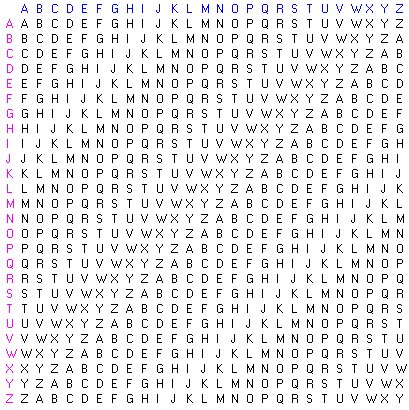
\includegraphics[scale=0.75]{../Image/matrice.jpg}
  % matrice.jpg: 409x410 pixel, 72dpi, 14.43x14.46 cm, bb=0 0 409 410
\end{center}

Exemple : Chiffrons le mot \texttt{Poney} à l'aide de la clé \texttt{EPITA} :\\
\texttt{Poney} \\
\texttt{EPITA} \\
\texttt{Poney} chiffré avec cette clé :
\begin{itemize}
\item P crypté avec la lettre E : T
\item O crypté avec la lettre P : D
\item N crypté avec la lettre I : V
\item E crypté avec la lettre T : X
\item Y crypté avec la lettre A : Y
\end{itemize}
\texttt{Poney} crypté à l'aide de la clé \texttt{EPITA} avec le chiffre de Vigenère donne \texttt{TDVXY} !

\subsection{Cryptage symétrique}

\subsubsection{DES}

\subsubsection{AES}

\subsection{Cryptage asymétrique}

\subsubsection{RSA}

Le RSA est un algorithme méthode de cryptographie inventée en 1977 par  Ron \textsc{Rivest}, Adi \textsc{Shamir} et Len \textsc{Adleman} (d'où le nom de RSA). C'est encore le système cryptographique à clé publique le plus utilisé de nos jours.

Petite anecdote : Au départ, \textsc{Rivest}, \textsc{Shamir} et \textsc{Adleman} voulaient prouver que tout système à clé plublique possède une faille, c'est ainsi qu'ils ont créé le RSA !

Son principe de fonctionnement suit 4 étapes :\\
Tout d'abord il y a la création des clés (que l'on nommera $P$, $Q$, $E$ et $D$). $P$ et $Q$ sont deux grands nombres premiers distincts. Leur génération se fait au hasard en utilisant un algorithme de test de primalité probabiliste. C'est un algorithme qui determine si un nombre est probablement premier selon le degré de probabilité que l'on a fixé dans l'algorithme. En cryptographie, on se \og contente \fg{} d'avoir un nombre dont on sait qu'il est premier avec une probabilité supérieur à $ 1 - \frac{1}{2^{100}} $. $E$ est un entier premier avec le produit $(P - 1)(Q - 1)$. $D$ est tel que $ED = 1 \textrm{ mod } (P - 1)(Q - 1)$ donc que $ED - 1$ est un multiple de $(P - 1)(Q - 1)$. On peut fabriquer $D$ à partir de $E$, $P$ et $Q$ en utilisant l'algorithme d'Euclide.

Ensuite il faut distribuer les clés. Le couple $(n, e)$ constitue la clé publique. Elle est disponible pour toute personne voulant crypter un message afin de nous l'envoyer ensuite. Le couple $(n, d)$ constitue notre clé privée que l'on garde secrète. Si une personne désire nous envoyer un message codé, elle le représente sous la forme de plusieurs entiers $M$ compris entre 0 et $n - 1$. Elle possède notre clé publique $(n, e)$ et calcule $C = M^{e} \textrm{ mod } n$. C'est ce dernier nombre qu'elle nous envoie.

Nous recevons donc $C$ et on calcule grâce à notre clé privée : $D = C^{d} \textrm{ mod } n$. D'après un théorème d'Euler $D = M^{de} = M \textrm{ mod } n$. On a donc reconstitué le message.

\section{Stéganographie}

\newpage

\part{Répartition des charges}
%descriptif précis
Nous allons coder le logiciel \emph{Nigma} qui permettra de crypter un fichier via un algorithme de cryptographie au choix puis l'incrustation dans une image par des méthodes de stéganographie. Ainsi, le fichier sera crypté puis camouflé dans une image quelconque. Il y a deux étapes importantes dans la réalisation du logiciel : le cryptage et la stéganographie. Nous considérons que les deux étapes sont liées.

Les langages de programmation que nous allons utiliser sont le \texttt{C} et le \texttt{Caml}. Notre programme sera compilé sous la distribution FreeBSD d'EPITA. Il possèdera un mode console ainsi qu'une interface graphique.

Nous allons coder la partie cryptographie majoritairement avec le langage \texttt{Caml} et la partie stéganographie majoritairement avec le langage \texttt{C}. Notre interface graphique sera quant à elle codée en \texttt{C}.

Les différentes parties de programmation sont réparties dans le groupe de la manière suivante :

\begin{tabular}{|l|c|c|c|c|}
  \hline
  Tâches              & Guillaume & Justin   & Stéphane & Sébastien \\ \hline \hline
  Cryptographie       & $\oplus$  &          &          & $\oplus$   \\ \hline
  Stéganographie      &           & $\oplus$ & $\oplus$ &           \\ \hline
  Interface Graphique &           & $\oplus$ & $\oplus$ &           \\ \hline
\end{tabular}

Cette répartition est à titre indicatif, chacun de nous compte en réalité s'intéresser et participer toutes ces tâches. Ainsi, selon notre avancée dans chaque partie, nous pourrons aider l'autre partie du groupe.

\newpage

\part{Planning de Réalisation}
%aligné sur les dates de soutenance
Pour la première soutenance, nous allons démarrer dans la partie cryptographie avec le cryptage RSA. Pour la stéganographie, nous coderons la création d'une image avec des niveaux de gris, le nuage de points sera organisé. Notre logiciel sera pour l'instant en mode console uniquement. Comme type fichier à crypter, nous nous occuperons excusivement d'un fichier texte afin de contrôler le cryptage et le décryptage plus facilement. Nous mettrons aussi en place notre site Web, il permettra de nous présenter ainsi que notre projet. L'intégralité du code source sera disponible au téléchargement.

Pour la deuxième soutenance, nous ajouterons le cryptage DES dans la partie cryptographie. L'utilisateur aura donc au choix les algorithmes de cryptage RSA et DES. Du côté de la stéganographie, nous présenterons notre progression de l'intégration d'un fichier dans une image. Nous aurons une interface graphique ou une utilisation en mode console au choix pour l'utilisateur. Nous diversifierons les types de fichier à crypter en ajoutant la possibilité d'utiliser une image.

Enfin, pour la soutenance finale, nous implémenterons l'algorithme de cryptage AES que nous ajouterons aux algorithmes déjà réalisés. La partie stéganographie sera terminée, nous aurons alors notre fichier crypté qui sera incrusté dans une image. Notre interface aura sans doute évoluée au regard de l'utilisation régulière que nous aurons testée.

Tout au long du projet, notre site Web sera mis à jour et décrira l'avancée du Projet Nigma.
\newpage

\part{Conclusion}

\newpage

\part*{Source}

\begin{itemize}
\item \href{http://www.bibmath.net/crypto/}{http://www.bibmath.net/crypto/}
\end{itemize}

\end{document}
